\documentclass[a4paper]{article}
\usepackage[pdftex]{graphicx}
\usepackage{anysize}
\marginsize{3cm}{3cm}{3cm}{3cm}
\linespread{1.2}
\usepackage[utf8]{inputenc}
\usepackage[T1]{fontenc}       
\usepackage[swedish]{babel}      
\usepackage{epstopdf}     % För svensk avstavning och svenska
\usepackage[osf]{mathpazo} % Palatino with smallcaps and oldstyle numbers
\usepackage[scaled]{helvet}
\usepackage{morefloats} %så att man kan ha fler float-bilder
%\restylefloat{table}
\usepackage{etoolbox}
\usepackage{hanging}
\usepackage{listings}
\usepackage{graphicx}
\usepackage[width=.75\textwidth]{caption} %så all bildtext blir smalare

\lstset{language=SQL}

\newcommand\getcurrentref[1]{%
 \ifnumequal{\value{#1}}{0}
  {??}
  {\the\value{#1}}%
}  
\newcommand\requirement[2]{
	\numberedrow{Krav}{#1}{#2}
}
\newcommand\scenario[2] {
	\numberedrow{Scenario}{#1}{#2}
}
\newcommand\numberedrow[3]{
	\noindent
	\textbf{#1 \getcurrentref{section}.\getcurrentref{subsection}.#2.} #3
	
}

\usepackage{fancyhdr}
\fancyhf{}
\fancyhead[L]{Ansvarig: SG}

\fancyhead[R]{Datum: \today | Version: 0.6 | Dokumentnummer: PUSS144404}


\title{STLDD - Software Top Level Design Document: NewPussSystem}                  	
\author{Systemarkitektgruppen \\ Nina Khayyami | Johan Rönnåker |Martin Lichota | Marcel Tovar Rascon}
\date{}

\begin{document}

\maketitle
\thispagestyle{fancy}
\tableofcontents
\newpage

\section*{Dokumenthistorik}

\begin{tabular}{ l l l p{8.5cm} }
Ver. & Datum & Ansv. & Beskrivning \\\hline
0.1 & 30 september 2014 & SG & Struktur för dokumentet\\
0.2 & 2 oktober 2014 & SG & Lagt in klass-diagram, ER-diagram, sekvens-diagram samt lagt in all text. Färdigt för informell granskning.\\
0.3 & 7 oktober 2014 & SG & Uppdaterat klassbeskrivningar, klassmetoder, klassdiagram, SQL-frågor, sessionsinformation, sekvensdiagram samt figurbeskrivningar.\\
0.4 & 7 oktober 2014 & SG & Uppdaterat enligt informella granskningsprotokollet.\\
0.5 & 7 oktober 2014 & SG & Uppdaterat klassdiagram, uppdaterat sekvensdiagram för klassen ProjectGroupAdmin, rättat stavfel och syntaxfel.\\
0.6 & 7 oktober 2014 & SG & Uppdaterat klassdiagram, sekvensdiagram och ett litet fel i metodbeskrivningen. 

\end{tabular}
\newpage
\section{Inledning}       
Dokumentet beskriver högnivådesignen för NewPussSystem tidrapporteringssystem.



\section{Referensdokument}
\begin{enumerate}
\item SRS - Software Requirements Specification (Dokumentnummer PUSS144401, version 0.21)
\item STLDD - Software Top Level Design Document: BaseBlockSystem (Dokumentnummer PUSS12004, version 1.0)
\end{enumerate}



\section{Sammanfattning}
Systemet är implementerat i en Tomcat server med följande klasser och klassmetoder:

\subsection{Klasser}
\begin{hangparas}{1.5em}{1}
\textbf{class servletBase} Den här klassen är superklass åt alla servlets i systemet. För beskrivning se sidan 2 i referensdokument 2.\end{hangparas} 

\vspace{5mm}
\begin{hangparas}{1.5em}{1}
\textbf{class Administration} Se sida 2 i referensdokument 2. En ändring har gjorts där metoden deleteUser ska returnera en boolean och inparametern ändras till (int id).\end{hangparas}

\vspace{5mm}
\begin{hangparas}{1.5em}{1}
\textbf{class LogIn} Se sida 2 i referensdokument 2.\end{hangparas}

\vspace{5mm}
\begin{hangparas}{1.5em}{1}
\textbf{class Access} Den här klassen använder sig av tabellen log och users i databasen för att hålla koll på vilka som är inloggade och aktiva. Har en användare varit inaktiv mer än 20 minuter, se dokumentreferens 1 krav 6.2.9, så nekar den åtkomst och loggar ut användaren. \end{hangparas}

\vspace{5mm}
\begin{hangparas}{1.5em}{1}
\textbf{class ProjectGroupAdmin} Den här servleten ärver från ServletBase. Först kontrollerar den att användaren har behörighet att besöka sidan. Om så är fallet presenteras en tabell med information om varje projektgrupp (namn, projektledare). I tabellen kan administratören välja att radera gruppen och att lägga till/radera en projektledare. Projektgruppsnamnet i tabellen länkar administratören till projektledarens ändringsmeny. Nedanför tabellen finns en meny där administratören kan välja att lägga till nya projektgrupper, lägga till/ta bort användare i projektgrupper, gå tillbaka till startsidan för administration, gå tillbaka till den gemensamma första inloggningssidan, samt logga ut.\end{hangparas}

\vspace{5mm}
\begin{hangparas}{1.5em}{1}
\textbf{class TimeReporting} Den här servleten ärver från ServletBase och presenterar en undermeny med menyval relaterade till tidrapportering. Förutom undermenyn kommer första sidan att vara tom. När ett val i undermenyn görs, kommer klassen att hantera den valda funktionen. Funktionerna som finns inkluderar att lista tidrapporter, visa och uppdatera tidrapporter samt skapa nya tidrapporter.\end{hangparas}

\vspace{5mm}
\begin{hangparas}{1.5em}{1}
\textbf{class ReportGenerator} Den här statiska klassen är en nästlad klass som har metoder som tar emot referenser till databasen och ritar upp en tidrapport med relevanta data. De olika tidrapporter som kan ritas upp är: en redigerbar, ny och tom tidrapport, en redigerbar existerande tidrapport och en icke redigerbar existerande tidrapport.\end{hangparas}

\vspace{5mm}
\begin{hangparas}{1.5em}{1}
\textbf{class ProjectLeader} Den här servleten ärver från ServletBase och visar en lista över alla användare. Härifrån kan projektledaren ändra projektmedlemmarnas roller. \end{hangparas}

\vspace{5mm}
\begin{hangparas}{1.5em}{1}
\textbf{class ReportHandling} Den här servleten ärver från ServletBase och visar två listor; en lista med signerade och en lista med osignerade tidrapporter om man väljer att hantera tidrapporter. Projektledaren kan här signera eller avsignera rapporter.\end{hangparas}

\vspace{5mm}
\begin{hangparas}{1.5em}{1}
\textbf{class Statistics} Den här servleten ärver från ServletBase och visar vissa funktioner om man väljer att generera statistik. Funktioner som kan väljas är t.ex. att visa vilken vecka som det har tidrapporterats mest tid.\\ \end{hangparas}

\subsection{Klassmetoder}
Nedan beskrivs alla klassmetoder till klasserna som presenterats under rubriken 3.1 Klasser.

\subsubsection{class Access}

\begin{hangparas}{1.5em}{1}
public boolean updateLog(int userID, String session)\\
Updates the log with a new timestamps for the given user and session. \\
@param userID: The requesting users id.\\
@param session: The requesting users session id.\\
@return boolean: True if the user has not been inactive for too long.
\end{hangparas}

\vspace{5mm}
\begin{hangparas}{1.5em}{1}
public boolean logInUser(int userID, String session)\\
Updates the database, sets the user as logged in, stores the current session id and current timestamp for the requesting user.\\
@param userID: The requesting users id.\\
@param session: The requesting users session id.\\
@return boolean: True if the user is not already logged in.
\end{hangparas}

\vspace{5mm}
\begin{hangparas}{1.5em}{1}
public boolean logOutUser(int userID, String session)\\
Updates the database, sets the user as logged out, removes the current session id and current timestamp for the requesting user.\\
@param userID: The requesting users id.\\
@param session: The requesting users session id.\\
@return boolean - True if the user is not already logged out.\\
\end{hangparas}

\subsubsection{class ProjectGroupAdmin}

\begin{hangparas}{1.5em}{1}
private String addProjectForm()\\
Constructs a form for adding project groups.\\
@return String - The html-code for constructing the form.
\end{hangparas}

\vspace{5mm}
\begin{hangparas}{1.5em}{1}
private boolean addProject(String name)\\
Adds a new project group. Has to be followed by a successful call of addUserToGroup(userID, groupID, role) with role = project leader.\\
@param name: The name of the new group.\\
@return boolean: True if the project is added successfully.
\end{hangparas}

\vspace{5mm}
\begin{hangparas}{1.5em}{1}
private boolean deleteProject(int projectID)\\
Deletes a project group.\\
@param projectID: The id of the project group which will be deleted.\\
@return boolean: True if the group is deleted successfully.
\end{hangparas}

\vspace{5mm}
\begin{hangparas}{1.5em}{1}
private boolean addUserToGroup(int userID, int groupID, String role)\\
Adds a user with a role to a group.\\
@param userID: The id of the user who will be added to the group.\\
@param groupID: The id of the group to which the user will be added to.\\
@param role: The role the user will have in the group.\\
@ return boolean: True if the user was successfully added.
\end{hangparas}

\vspace{5mm}
\begin{hangparas}{1.5em}{1}
private boolean removeUserFromGroup(int userGroupID)\\
Removes the user from the group. Which user and group are found in the database's tabel user\_group.\\
@param userGroupID: The ID of the row in the table user\_group on which the user and group can be found.\\
@return boolean: True if the user was successfully removed.\\
\end{hangparas}


\subsubsection{class TimeReporting}

\begin{hangparas}{1.5em}{1}
private void viewReportList(int userID)\\
Prints out a list of the user’s own reports. \\
@param userID: The id of the user.
\end{hangparas}

\vspace{5mm}
\begin{hangparas}{1.5em}{1}
private void viewReport(int reportID)\\
Fetches the data for the time report specified by the reportID parameter and passes the data on to the static method viewReport in the static ReportGenerator class.\\
@param reportID: The id of the time report.
\end{hangparas}

\vspace{5mm}
\begin{hangparas}{1.5em}{1}
private void printUpdateReport(int reportID)\\
Fetches the data for the time report specified by the reportID parameter and passes the data on to the static method updateReport in the static ReportGenerator class.\\
@param reportID: The id of the time report.
\end{hangparas}

\vspace{5mm}
\begin{hangparas}{1.5em}{1}
private void printNewReport(int weekNumber)\\
Prints out the new timereport html-form.\\
@param weekNumber: The weeknumber for the time report.
\end{hangparas}

\vspace{5mm}
\begin{hangparas}{1.5em}{1}
private void updateReport(int reportID)\\
Updates the data stored in the database for the report specified by the reportID parameter.\\
@param reportID: The id of the time report to update. 
\end{hangparas}

\vspace{5mm}
\begin{hangparas}{1.5em}{1}
private void deleteReport(int reportID)\\
Deletes the report specified by the reportID parameter after confirmation and if and only if it is unsigned.\\
@param reportID: The id of the time report to delete.
\end{hangparas}

\vspace{5mm}
\begin{hangparas}{1.5em}{1}
private void addNewReport()\\
Inserts the data from the new report form into the database.
\end{hangparas}

\vspace{5mm}
\begin{hangparas}{1.5em}{1}
private void filterReportList(String filter)\\
Filters what time reports that should be shown in the list.\\
@param filter: The filter that should be applied.\\
\end{hangparas}


\subsubsection{class ReportGenerator}

\begin{hangparas}{1.5em}{1}
public static void viewReport(ResultSet data)\\
Prints out a time report in the right format and with the data specified by the ResultSet parameter.\\
@param data: Specifies which data to print in the time report. 
\end{hangparas}

\vspace{5mm}
\begin{hangparas}{1.5em}{1}
public static void updateReport(ResultSet data)\\
Prints out a html-form in the right format and with the data specified by the ResultSet parameter.\\ 
@param data: Specifies which data to print in the html-form.
\end{hangparas}

\vspace{5mm}
\begin{hangparas}{1.5em}{1}
public static void newReport(int weekNumber)\\
Prints out a time report html-form prefilled with data.\\
@param weekNumber: Specifies for which week the data should be shown.\\
\end{hangparas}
 

\subsubsection{class ProjectLeader}

\begin{hangparas}{1.5em}{1}
public void showAllUsers(int groupID)\\
Shows a list of all the users in the system.\\
@param groupID: The group which members should be listed.
\end{hangparas}

\vspace{5mm}
\begin{hangparas}{1.5em}{1}
public boolean changeRole(int userGroupID, String role)\\
Assigns a role to a user in a project group.\\
@param userGroupID: The user to be assigned a role, and in which group.\\
@param role: Which role to assign.\\
@return boolean: True if the user was successfully added.\\
\end{hangparas}

\subsubsection{class ReportHandling}

\begin{hangparas}{1.5em}{1}
private boolean signTimeReport(int timeReportID)\\
Signs a time report.\\
@param timeReportID: The id of the report that will be signed.\\
@return boolean: True if the time report was successfully signed.
\end{hangparas}

\vspace{5mm}
\begin{hangparas}{1.5em}{1}
private boolean unsignTimeReport(int timeReportID)\\
Unsigns a time report.\\
@param timeReportID: The id of the report that will be unsigned.\\
@return boolean: True if the time report was succcessfully unsigned.
\end{hangparas}

\vspace{5mm}
\begin{hangparas}{1.5em}{1}
private void showAllReports(int group)\\
Shows a list of all the time reports, from the specified group with the given id.\\
@param group: The project leaders group id.\\
\end{hangparas}


\subsubsection{class Statistics}

\begin{hangparas}{1.5em}{1}
private boolean generateStatisticsReport(int groupID, int userID, String role, String weeks, String activity)\\
Shows a time report based on the parameters requested by the user.\\
@param groupID: The project leaders group id.\\
@param userID: The user for the time report.\\
@param role: The role of the user(s) for the time report.\\
@param weeks: The weeks for which the time report will be shown.\\
@param activity: The activity that will be included in the time report.\\
@return boolean: True if the report was successfully generated and shown.
\end{hangparas}

\vspace{5mm}
\begin{hangparas}{1.5em}{1}
private boolean generateSummarizedReport(List<String> timeReports, String activity, String subactivity)\\
Shows a time report with the summarized activity from several time reports.\\
@param timeReports: The time reports which it will summarize from.\\
@param activity: The activity which will be summarized.\\
@param subactivity: The subactivity which will be summarized.\\
@return boolean: True if the time report was successfully generated.
\end{hangparas}

\vspace{5mm}
\begin{hangparas}{1.5em}{1}
private String commonActivity(int groupID)\\
Finds the activity that has the most combined minutes reported by the users in the project group.\\
@param groupID: The project leaders group id.\\
@return string: Returns the activity.
\end{hangparas}

\vspace{5mm}
\begin{hangparas}{1.5em}{1}
private int busiestWeek(int groupID)\\
Finds the week with the most combined minutes reported by the users in the project group.\\
@param groupID: The project leaders group id.\\
@return int: Returns the busiest week.\\
\end{hangparas}

\section{Klassdiagram}
Ett klassdiagram med alla klasser visas i Figur \ref{umldiagram}.

\begin{figure}[h!]
\centering
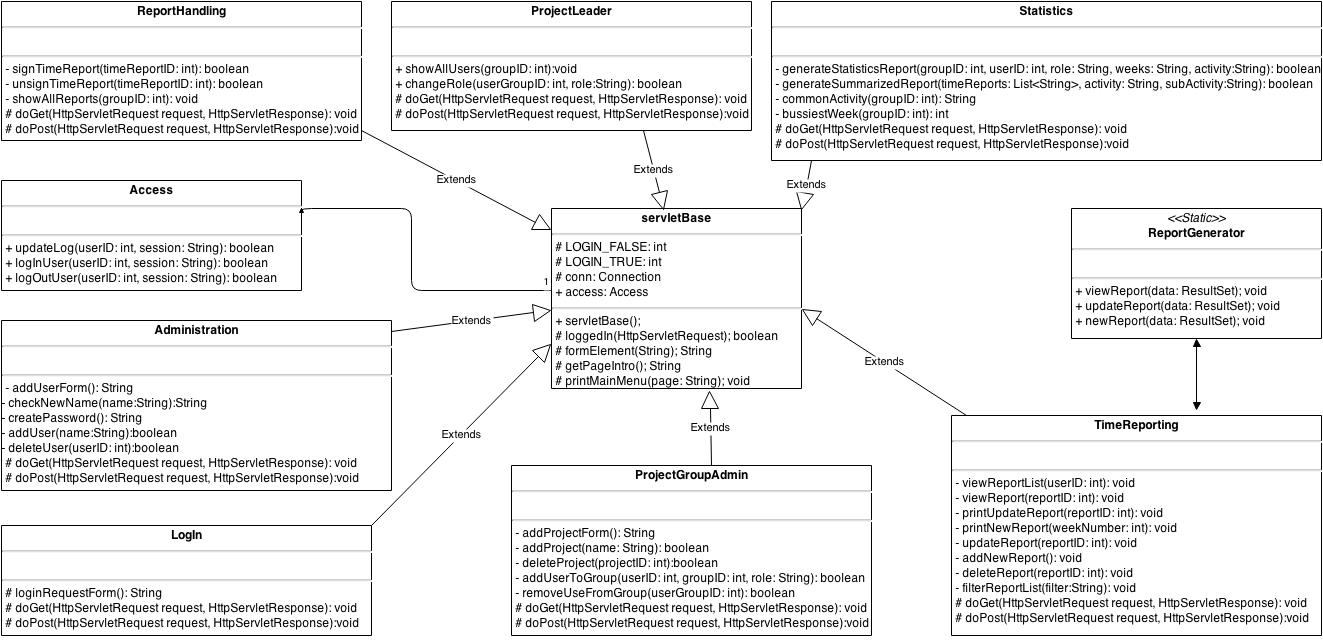
\includegraphics[width=160mm]{UML.jpg}
\caption{Klassdiagram över alla klasser i systemet. \label{umldiagram}}
\end{figure}



\section{Databas}

ER-diagram över databasen för systemet visas i figur \ref{ER}. Databasen kan skapas från scratch med följande SQL kommandon: \\

\begin{figure}[ht!]
\centering
\includegraphics[width=120mm]{DB__1___9_.png}
\caption{ER-diagram över databasen för systemet \label{ER}}
\end{figure}

\begin{lstlisting}
mysql> create database base;
mysql> use base;

mysql> CREATE TABLE IF NOT EXISTS `groups` (
    ->   `id` int(11) NOT NULL AUTO_INCREMENT,
    ->   `name` varchar(20) NOT NULL,
    ->   PRIMARY KEY (`id`),
    ->   UNIQUE KEY `name` (`name`)
    -> ) ENGINE=InnoDB DEFAULT CHARSET=utf8 AUTO_INCREMENT=1 ;

mysql> CREATE TABLE IF NOT EXISTS `log` (
    ->   `id` int(11) NOT NULL AUTO_INCREMENT,
    ->   `user_id` int(11) NOT NULL,
    ->   `time` timestamp NOT NULL DEFAULT CURRENT_TIMESTAMP ON UPDATE
    ->     CURRENT_TIMESTAMP,
    ->   `session` varchar(100) NOT NULL,
    ->   PRIMARY KEY (`id`),
    ->   KEY `user_id` (`user_id`)
    -> ) ENGINE=InnoDB DEFAULT CHARSET=utf8 AUTO_INCREMENT=1 ;

mysql> CREATE TABLE IF NOT EXISTS `reports` (
    ->   `id` int(11) NOT NULL AUTO_INCREMENT,
    ->   `user_group_id` int(11) NOT NULL,
    ->   `date` date NOT NULL,
    ->   `week` int(11) NOT NULL,
    ->   `total_time` int(11) NOT NULL,
    ->   `signed` tinyint(4) NOT NULL,
    ->   PRIMARY KEY (`id`),
    ->   KEY `user_group_id` (`user_group_id`)
    -> ) ENGINE=InnoDB DEFAULT CHARSET=utf8 AUTO_INCREMENT=1 ;
    
mysql> CREATE TABLE IF NOT EXISTS `report_times` (
    ->   `id` int(11) NOT NULL AUTO_INCREMENT,
    ->   `report_id` int(11) NOT NULL,
    ->   `SDP_U` int(11) NOT NULL,
    ->   `SDP_I` int(11) NOT NULL,
    ->   `SDP_F` int(11) NOT NULL,
    ->   `SDP_O` int(11) NOT NULL,
    ->   `SRS_U` int(11) NOT NULL,
    ->   `SRS_I` int(11) NOT NULL,
    ->   `SRS_F` int(11) NOT NULL,
    ->   `SRS_O` int(11) NOT NULL,
    ->   `SVVS_U` int(11) NOT NULL,
    ->   `SVVS_I` int(11) NOT NULL,
    ->   `SVVS_F` int(11) NOT NULL,
    ->   `SVVS_O` int(11) NOT NULL,
    ->   `STLDD_U` int(11) NOT NULL,
    ->   `STLDD_I` int(11) NOT NULL,
    ->   `STLDD_F` int(11) NOT NULL,
    ->   `STLDD_O` int(11) NOT NULL,
    ->   `SVVI_U` int(11) NOT NULL,
    ->   `SVVI_I` int(11) NOT NULL,
    ->   `SVVI_F` int(11) NOT NULL,
    ->   `SVVI_O` int(11) NOT NULL,
    ->   `SDDD_U` int(11) NOT NULL,
    ->   `SDDD_I` int(11) NOT NULL,
    ->   `SDDD_F` int(11) NOT NULL,
    ->   `SDDD_O` int(11) NOT NULL,
    ->   `SVVR_U` int(11) NOT NULL,
    ->   `SVVR_I` int(11) NOT NULL,
    ->   `SVVR_F` int(11) NOT NULL,
    ->   `SVVR_O` int(11) NOT NULL,
    ->   `SSD_U` int(11) NOT NULL,
    ->   `SSD_I` int(11) NOT NULL,
    ->   `SSD_F` int(11) NOT NULL,
    ->   `SSD_O` int(11) NOT NULL,
    ->   `slutrapport_U` int(11) NOT NULL,
    ->   `slutrapport_I` int(11) NOT NULL,
    ->   `slutrapport_F` int(11) NOT NULL,
    ->   `slutrapport_O` int(11) NOT NULL,
    ->   `funktionstest` int(11) NOT NULL,
    ->   `systemtest` int(11) NOT NULL,
    ->   `regressionstest` int(11) NOT NULL,
    ->   `meeting` int(11) NOT NULL,
    ->   `lecture` int(11) NOT NULL,
    ->   `excersice` int(11) NOT NULL,
    ->   `terminal` int(11) NOT NULL,
    ->   `study` int(11) NOT NULL,
    ->   `other` int(11) NOT NULL,
    ->   PRIMARY KEY (`id`),
    ->   KEY `report_id` (`report_id`)
    -> ) ENGINE=InnoDB DEFAULT CHARSET=utf8 AUTO_INCREMENT=1 ;

mysql> CREATE TABLE IF NOT EXISTS `users` (
    ->   `id` int(11) NOT NULL AUTO_INCREMENT,
    ->   `username` varchar(10) NOT NULL,
    ->   `password` varchar(10) NOT NULL,
    ->   `is_admin` tinyint(4) NOT NULL,
    ->   `is_project_leader` tinyint(4) NOT NULL,
    ->   `is_logged_in` tinyint(4) NOT NULL,
    ->   PRIMARY KEY (`id`),
    ->   UNIQUE KEY `username` (`username`)
    -> ) ENGINE=InnoDB DEFAULT CHARSET=utf8 AUTO_INCREMENT=1 ;
    
mysql> CREATE TABLE IF NOT EXISTS `user_group` (
    ->   `id` int(11) NOT NULL AUTO_INCREMENT,
    ->   `user_id` int(11) NOT NULL,
    ->   `group_id` int(11) NOT NULL,
    ->   `role` varchar(20) NOT NULL,
    ->   PRIMARY KEY (`id`),
    ->   KEY `user_id` (`user_id`),
    ->   KEY `group_id` (`group_id`)
    -> ) ENGINE=InnoDB DEFAULT CHARSET=utf8 AUTO_INCREMENT=1 ;
    
mysql> ALTER TABLE `log`
    ->   ADD CONSTRAINT `log_ibfk_1` FOREIGN KEY (`user_id`) REFERENCES `users`
    ->   (`id`);

mysql> ALTER TABLE `reports`
    ->   ADD CONSTRAINT `reports_ibfk_1` FOREIGN KEY (`user_group_id`) REFERENCES
    ->   `user_group` (`id`);

mysql> ALTER TABLE `report_times`
    ->   ADD CONSTRAINT `report_times_ibfk_1` FOREIGN KEY (`report_id`) REFERENCES
    ->   `reports` (`id`);

mysql> ALTER TABLE `user_group`
    ->   ADD CONSTRAINT `user_group_ibfk_2` FOREIGN KEY (`group_id`) REFERENCES
    ->    `groups`  (`id`),
    ->  ADD CONSTRAINT `user_group_ibfk_1` FOREIGN KEY (`user_id`) REFERENCES
    ->    `users`  (`id`);
  
\end{lstlisting}


\section{Information lagrad i sessioner}
I en pågående session sparas följande attribut i sessionen:

\vspace{5mm}
\begin{hangparas}{1.5em}{1}
\textbf{Session session}: Användarens sessions-id.
\end{hangparas}

\vspace{5mm}
\begin{hangparas}{1.5em}{1}
\textbf{String name}: Användarens användarnamn, e.g. 'admin'. 
\end{hangparas}

\vspace{5mm}
\begin{hangparas}{1.5em}{1}
\textbf{int userID}: Användarens id. 
\end{hangparas}

\vspace{5mm}
\begin{hangparas}{1.5em}{1}
\textbf{int userGroupID}: Id som säger vilken grupp användaren är inloggad för. 
\end{hangparas}

\section{Sekvensdiagram}

Observera att inte alla meddelanden visas i följande sekvensdiagram, utan endast de meddelanden som krävs för att förstå sekvensen.

\subsection{class Administration}
Figur 2 i dokumentreferens 2 visar sekvensen för hur servleten Administration hanterar att administratören lägger till en ny användare.


\subsection{class ProjectGroupAdmin}
Figur \ref{addGroup} visar hur servleten ProjectGroupAdmin hanterar en förfrågan om att lägga till en ny projektgrupp och Figur \ref{addGroupFail} visar hur den hanteras när den misslyckas. 

\begin{figure}[h!]
\centering
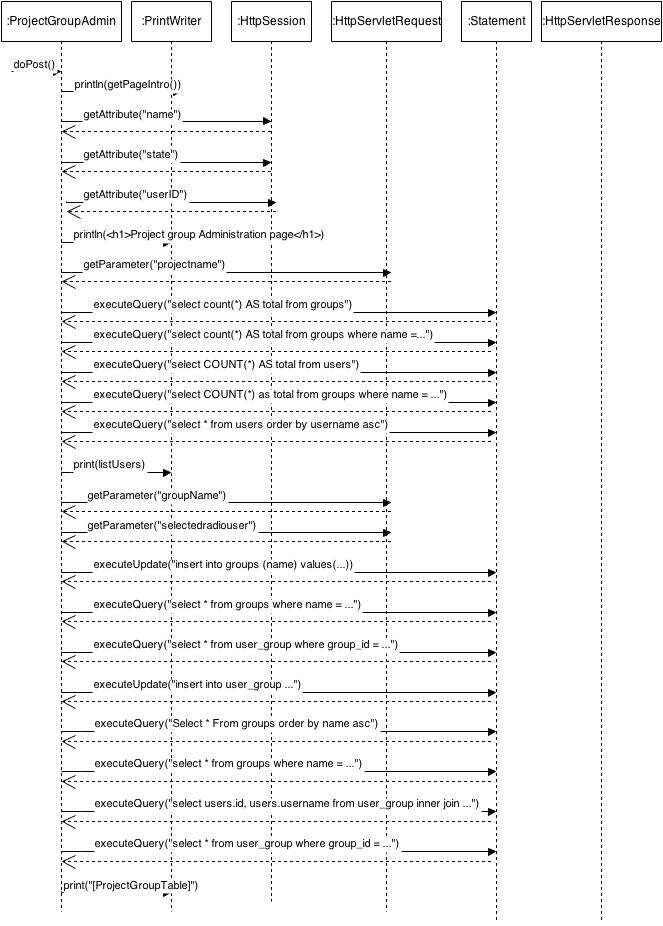
\includegraphics[width=90mm]{SeqDia__addGroup_FINAL.jpg}
\caption{Sekvensdiagram som visar hur en lyckad förfrågan om att lägga till en ny projektgrupp hanteras i klassen ProjectGroupAdmin. \label{addGroup}}
\end{figure}

\begin{figure}[h!]
\centering
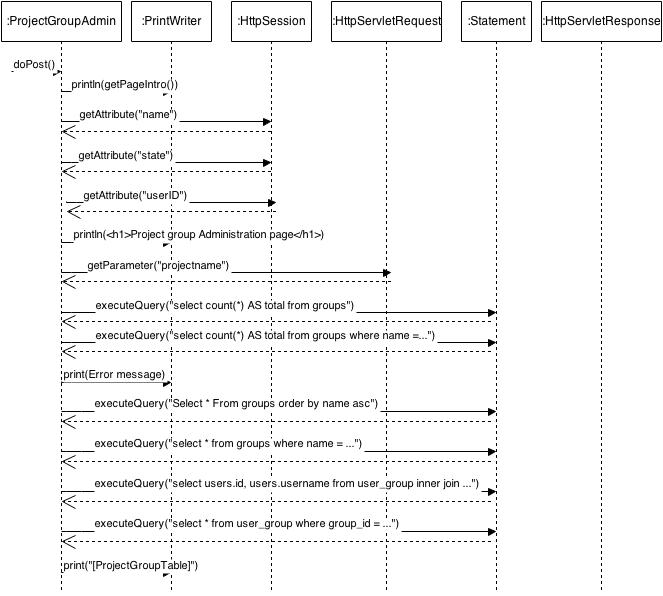
\includegraphics[width=90mm]{SeqDia__addGroup_Fail_FINAL.jpg}
\caption{Sekvensdiagram som visar hur en misslyckad förfrågan om att lägga till en ny projektgrupp hanteras i klassen ProjectGroupAdmin. \label{addGroupFail}}
\end{figure}

\noindent
Figur \ref{addUserToGroup} visar hur servleten ProjectGroupAdmin hanterar en förfrågan om att lägga till en användare i en projektgrupp, medan Figur \ref{addUserToGroupFail} visar hur det hanteras när den misslyckas.

\begin{figure}[h!]
\centering
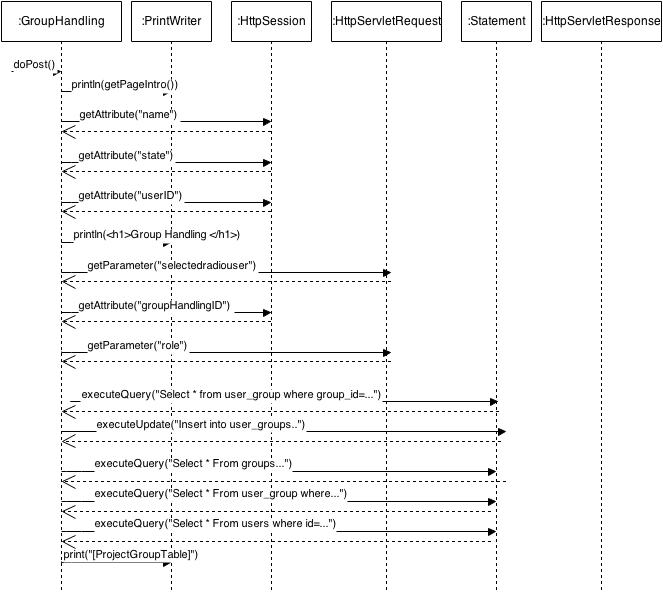
\includegraphics[width=90mm]{SeqDia__addUserToGroup_FINAL.jpg}
\caption{Sekvensdiagram som visar hur klassen ProjectGroupAdmin hanterar en förfrågan om att lägga till en användare i en projektgrupp.
\label{addUserToGroup}}
\end{figure}

\begin{figure}[h!]
\centering
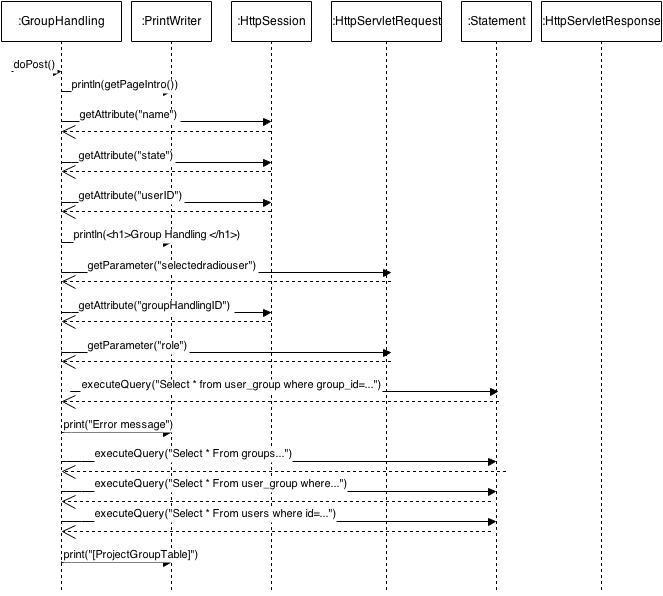
\includegraphics[width=90mm]{SeqDia__addUserToGroup_Fail_FINAL.jpg}
\caption{Sekvensdiagram som visar hur klassen ProjectGroupAdmin hanterar en misslyckad förfrågan om att lägga till en användare i en projektgrupp.
\label{addUserToGroupFail}}
\end{figure}

\noindent
Figur \ref{removeUserFromGroup} visar hur servleten ProjectGroupAdmin hanterar en förfrågan om att ta bort en användare från en projektgrupp, medan Figur \ref{removeUserFromGroupFail} visar hur det hanteras när den misslyckas.

\begin{figure}[h!]
\centering
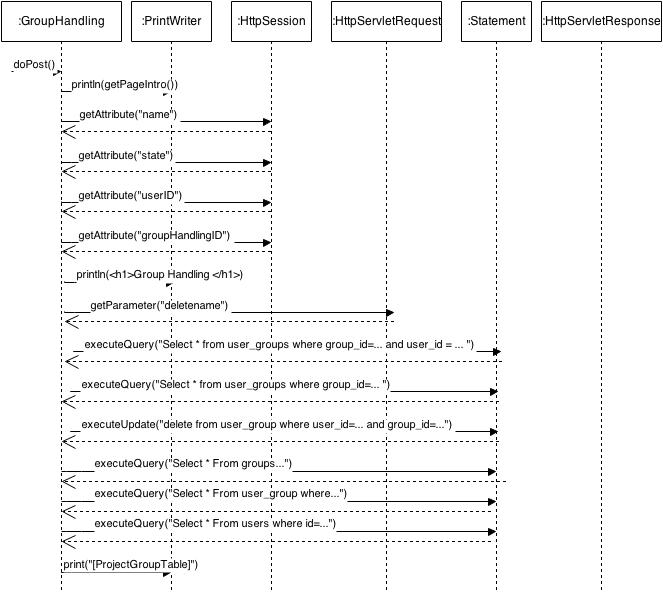
\includegraphics[width=90mm]{SeqDia__removeUserFromGroup_FINAL.jpg}
\caption{Sekvensdiagram som visar hur klassen ProjectGroupAdmin hanterar en förfrågan om att ta bort en användare från en projektgrupp.
\label{removeUserFromGroup}}
\end{figure}

\begin{figure}[h!]
\centering
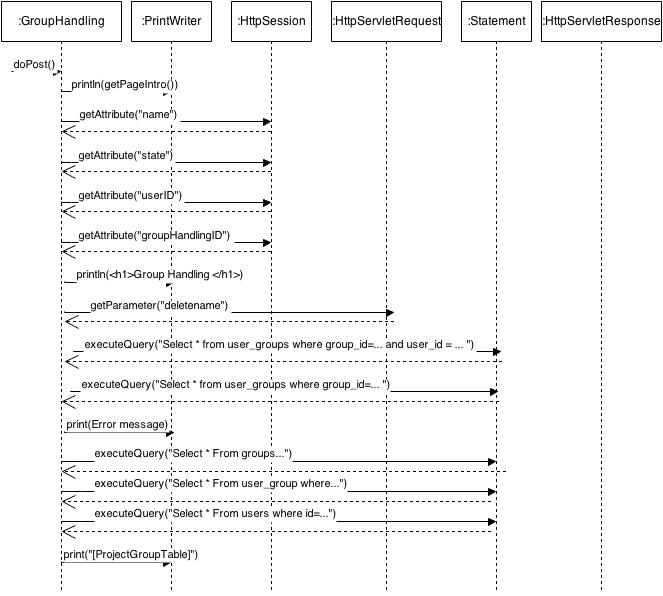
\includegraphics[width=90mm]{SeqDia__removeUserFromGroup_Fail_FINAL.jpg}
\caption{Sekvensdiagram som visar hur klassen ProjectGroupAdmin hanterar en misslyckad förfrågan om att ta bort en användare från en projektgrupp.
\label{removeUserFromGroupFail}}
\end{figure}

\noindent
Figur \ref{removeGroup} visar hur servleten ProjectGroupAdmin hanterar en förfrågan om att ta bort en projektgrupp.

\begin{figure}[h!]
\centering
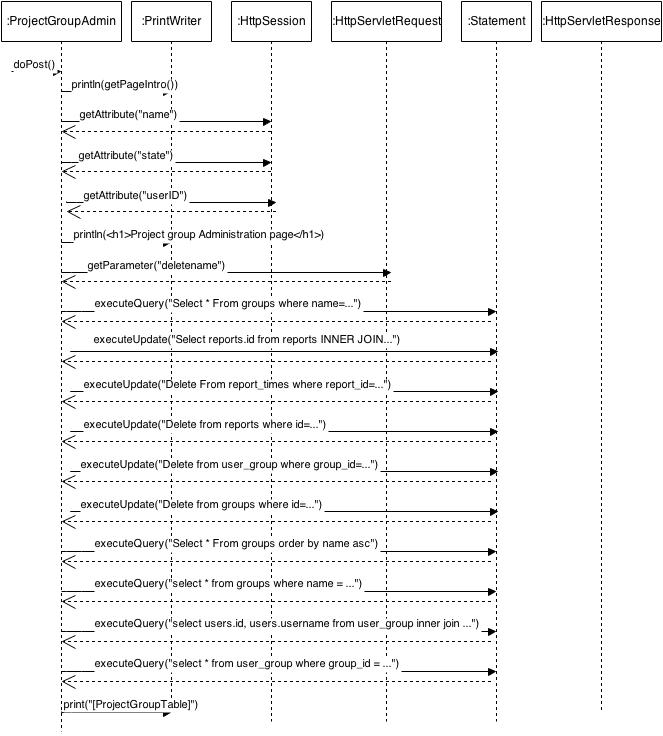
\includegraphics[width=90mm]{SeqDia__removeGroup_FINAL.jpg}
\caption{Sekvensdiagram som visar hur klassen ProjectGroupAdmin hanterar en förfrågan om att ta bort en projektgrupp.
\label{removeGroup}}
\end{figure}

\subsection{TimeReporting}
Figur \ref{newReport} visar hur servleten TimeReporting hanterar en förfrågan om att skapa en ny tidrapport som läggs till i databasen.

\begin{figure}[h!]
\centering
\includegraphics[width=90mm]{newReport_successful.jpg}
\caption{Visar sekvensen av de grundläggande metodanrop som sker då användaren framgångsrikt skapar en ny tidrapport i klassen TimeReporting.
\label{newReport}}
\end{figure}

\noindent
Figur \ref{removeReport} visar hur servleten TimeReporting hanterar en förfrågan om att ta bort en tidrapport och Figur \ref{removeReportFail} visar hur det hanteras när den misslyckas.

\begin{figure}[h!]
\centering
\includegraphics[width=90mm]{removeReport_successful.jpg}
\caption{Visar sekvensen av de grundläggande metodanrop som sker i klassen TimeReporting då användaren framgångsrikt tar bort en tidrapport som inte är signerad.
\label{removeReport}}
\end{figure}

\begin{figure}[h!]
\centering
\includegraphics[width=90mm]{removeReport_unsuccessful.jpg}
\caption{Visar sekvensen av de grundläggande metodanrop som sker i klassen TimeReporting då användaren misslyckat försöker ta bort en tidrapport som är signerad.
\label{removeReportFail}}
\end{figure}

\noindent
Figur \ref{updateReportSigned} visar hur servleten TimeReporting hanterar en förfrågan om att uppdatera en tidrapport som redan blivit signerad och Figur \ref{updateReportUnsigned} visar hur en förfrågan om att uppdatera en tidrapport som ännu inte blivit signerad hanteras.

\begin{figure}[h!]
\centering
\includegraphics[width=90mm]{updateReport_signed.jpg}
\caption{Visar sekvensen av de grundläggande metodanrop som sker i klassen TimeReporting då användaren misslyckat försöker uppdatera en tidrapport som är signerad.
\label{updateReportSigned}}
\end{figure}

\begin{figure}[h!]
\centering
\includegraphics[width=90mm]{updateReport_unsigned.jpg}
\caption{Visar sekvensen av de grundläggande metodanrop som sker i klassen TimeReporting då användaren framgångsrikt uppdaterar en tidrapport som inte är signerad.
\label{updateReportUnsigned}}
\end{figure}

\noindent
Figur \ref{viewReportList} visar hur servleten TimeReporting hanterar en förfrågan om att skriva ut en användares alla tidrapporter, Figur \ref{viewReportListFail} visar hur den hanteras när den misslyckas.

\begin{figure}[h!]
\centering
\includegraphics[width=90mm]{viewReportList_successful.jpg}
\caption{Visar sekvensen av de grundläggande metodanrop som sker i klassen TimeReporting då användaren framgångsrikt listar alla sina befintliga tidrapporter.
\label{viewReportList}}
\end{figure}

\begin{figure}[h!]
\centering
\includegraphics[width=90mm]{viewReportList_unsuccessful.jpg}
\caption{Visar sekvensen av de grundläggande metodanrop som sker i klassen TimeReporting då användaren misslyckat försöker lista alla sina befintliga tidrapporter, då denne inte har några befintliga tidrapporter.
\label{viewReportListFail}}
\end{figure}


\subsection{ProjectLeader}
Figur \ref{assignRole} visar hur servleten ProjectLeader hanterar en förfrågan om att ändra en projektroll för en användare.

\begin{figure}[h!]
\centering
\includegraphics[width=90mm]{assignRole.jpg}
\caption{Sekvensdiagram som beskriver hur klassen ProjectLeader hanterar en förfrågan om att ändra en projektroll för en användare.
\label{assignRole}}
\end{figure}

\subsection{ReportHandling}

Figur \ref{showAllViewReport} visar hur servleten ReportHandling hanterar en förfrågan om att visa alla tidrapporter i projektgruppen, signerade samt osignerade. Figur \ref{signedReport} visar hur servleten ProjectLeader hanterar en förfrågan om att signera en rapport.

\begin{figure}[h!]
\centering
\includegraphics[width=90mm]{showAllViewReport.jpg}
\caption{Sekvensdiagram som visar hur klassen ReportHandling hanterar en förfrågan om att visa alla tidrapporter i en projektgrupp.
\label{showAllViewReport}}
\end{figure}

\begin{figure}[h!]
\centering
\includegraphics[width=90mm]{signedReport.jpg}
\caption{Sekvensdiagram som visar hur klassen ReportHandling hanterar en förfrågan om att signera en rapport.
\label{signedReport}}
\end{figure}

\subsection{Statistics}
Figur \ref{busiestWeek} visar hur servleten Statistics hanterar en förfrågan om att visa vilken vecka som har flest totala inlagda minuter.\\
Figur \ref{commonActivity} visar hur servleten Statistics hanterar en förfrågan om att visa vilken aktivitet som har flest totala inlagda minuter.\\
Figur \ref{generateStatisticsReport} visar hur servleten Statistics hanterar en förfrågan om att visa en tidrapport som sammanfattar arbetet utfört i en viss aktivitet av en viss grupp/undergrupp under en specifik tid.

\begin{figure}[h!]
\centering
\includegraphics[width=90mm]{busiestWeek.jpg}
\caption{Sekvensdiagram som visar hur en förfrågan om att visa vilken vecka som har flest totala inlagda minuter hanteras i klassen Statistics.
\label{busiestWeek}}
\end{figure}

\begin{figure}[h!]
\centering
\includegraphics[width=90mm]{commonActivity.jpg}
\caption{Sekvensdiagram som beskriver hur en förfrågan om att visa vilken aktivitet som har flest totala inlagda minuter hanteras i klassen Statistics.
\label{commonActivity}}
\end{figure}

\begin{figure}[h!]
\centering
\includegraphics[width=90mm]{generateStatisticsReport.jpg}
\caption{Sekvensdiagram som visar hur klassen Statistics hanterar en förfrågan om att visa en tidrapport som sammanfattar arbetet utfört i en viss aktivitet av en viss grupp/undergrupp under en specifik tid.
\label{generateStatisticsReport}}
\end{figure}

\end{document}